\documentclass[defesa,oneside,brazilian,english]{ppginf}

% Pacotes usados neste documento e suas respectivas configurações

% ------------------------------------------------------------------------------

% Definição de fontes

% formato dos arquivos-fonte (utf8 no Linux e latin1 no Windows)
\usepackage[utf8]{inputenc}	% arquivos LaTeX em Unicode (UTF8)

% usar codificação T1 para ter caracteres acentuados corretos no PDF

% fonte usada no corpo do texto (pode alterar, mas descomente apenas uma)
%\usepackage{newtxtext,newtxmath}	% Times (se não tiver, use mathptmx)
%\usepackage{lmodern}			% Computer Modern (fonte clássico LaTeX)
\usepackage{kpfonts}			% Kepler/Palatino (idem, use mathpazo)
%\renewcommand{\familydefault}{\sfdefault} % Arial/Helvética (leia abaixo)

% A biblioteca central da UFPR recomenda usar Arial, seguindo a recomendação da
% ABNT. Essa é uma escolha ruim, pois fontes sans-serif são geralmente inade-
% quados para textos longos e impressos, sendo melhores para páginas Web.
% http://www.webdesignerdepot.com/2013/03/serif-vs-sans-the-final-battle/.

% fontes usadas em ambientes específicos
\usepackage[scaled=0.9]{helvet}		% Sans Serif
\usepackage{courier}			% Verbatim, Listings, etc

% ------------------------------------------------------------------------------

% inclusão de figuras em PDF, PNG, PS, EPS
\usepackage{graphicx}

% subfiguras (subfigure is deprecated, don't use it)
\usepackage[labelformat=simple]{subcaption}
\renewcommand\thesubfigure{(\alph{subfigure})}

% ------------------------------------------------------------------------------

% inclusão/formatação de código-fonte (programas)
\usepackage{listings}
\lstset{language=c}
\lstset{basicstyle=\ttfamily\footnotesize,commentstyle=\textit,stringstyle=\ttfamily}
\lstset{showspaces=false,showtabs=false,showstringspaces=false}
\lstset{numbers=left,stepnumber=1,numberstyle=\tiny}
\lstset{columns=flexible,mathescape=true}
\lstset{frame=single}
\lstset{inputencoding=utf8,extendedchars=true}
\lstset{literate={á}{{\'a}}1  {ã}{{\~a}}1 {à}{{\`a}}1 {â}{{\^a}}1
                 {Á}{{\'A}}1  {Ã}{{\~A}}1 {À}{{\`A}}1 {Â}{{\^A}}1
                 {é}{{\'e}}1  {ê}{{\^e}}1 {É}{{\'E}}1  {Ê}{{\^E}}1
                 {í}{{\'\i}}1 {Í}{{\'I}}1
                 {ó}{{\'o}}1  {õ}{{\~o}}1 {ô}{{\^o}}1
                 {Ó}{{\'O}}1  {Õ}{{\~O}}1 {Ô}{{\^O}}1
                 {ú}{{\'u}}1  {Ú}{{\'U}}1
                 {ç}{{\c{c}}}1 {Ç}{{\c{C}}}1 }

% ------------------------------------------------------------------------------

% formatação de algoritmos
\usepackage{algorithm,algorithmic}
%\IfLanguageName{brazilian} {\floatname{algorithm}{Algoritmo}}{}
\renewcommand{\algorithmiccomment}[1]{~~~// #1}
%\algsetup{linenosize=\footnotesize,linenodelimiter=.}

% ------------------------------------------------------------------------------

% formatação de bibliografia
\usepackage{natbib}			% bibliografia no estilo NatBib
% \IfLanguageName{brazilian}
% {\bibliographystyle{apalike-ptbr}}	% formato em português
% {\bibliographystyle{apalike}}		% formato em inglês

% Estilos de bibliografia recomendados (só descomentar um estilo!)
% Mais infos: https://pt.sharelatex.com/learn/Bibtex_bibliography_styles
%
%\bibliographystyle{apalike-ptbr}	% [Maziero et al., 2006]
%\bibliographystyle{alpha}		% [Maz06]
%\bibliographystyle{plainnat}		% vide Google "LaTeX Natbib"
%\bibliographystyle{plain}		% [1] ordem alfabética
\bibliographystyle{unsrt}		% [1] ordem de uso no texto

% no estilo "unsrt", evita que citações nos índices sejam consideradas
%\usepackage{notoccite}

\renewcommand{\cite}{\citep}	% \cite deve funcionar como \citep
%\bibpunct{[}{]}{;}{a}{}{,}	% caracteres usados nas referências

% ------------------------------------------------------------------------------

% fontes adicionais
\usepackage{amsmath}		% pacotes matemáticos
\usepackage{amsfonts}		% fontes matemáticas 
%\usepackage{amssymb}		% símbolos 

% ------------------------------------------------------------------------------

% pacotes diversos
\usepackage{alltt,moreverb}	% mais comandos no modo verbatim
\usepackage{lipsum}		% gera texto aleatório (para os exemplos)
\usepackage{currfile}		% infos sobre o arquivo/diretório atual
\usepackage[final]{pdfpages}	% inclusão de páginas em PDF
\usepackage{longtable}		% tabelas multi-páginas (tab símbolos/acrônimos)

% CUSTOM PACKAGES ADDED BY GABRIEL HISHIDA
\usepackage{xcolor,colortbl}
\usepackage{notoccite}
% ------------------------------------------------------------------------------



\makeatletter
\g@addto@macro\@floatboxreset{\centering}
\makeatother
% Language setting
% Replace `english' with e.g. `spanish' to change the document language
%\usepackage[brazilian]{babel}

% Set page size and margins
% Replace `letterpaper' with `a4paper' for UK/EU standard size
%\usepackage[letterpaper,top=2cm,bottom=2cm,left=3cm,right=3cm,marginparwidth=1.75cm]{geometry}

% Useful packages
\usepackage{amsmath}
\usepackage{graphicx}
\usepackage{bm}
\usepackage{tikz}
\usetikzlibrary{arrows.meta}
%\usepackage{float}


%\usepackage[colorlinks=true, allcolors=blue]{hyperref}

\begin{document}



\title{Analise crítica dos limites do Blockchain em relacão a escalabilidade e capacidade de processamento de transacões em grande escala}
\author{Kokouvi Hola Kanyi Kodjovi}
\advisor{Eduardo Todt}

% instituição
\IfLanguageName{brazilian}
  { \instit{UFPR}{Universidade Federal do Paraná} }
% a Bib/UFPR exige que tudo seja em português, exceto o título :-(
%  { \instit{UFPR}{Federal University of Paraná} }
  { \instit{UFPR}{Universidade Federal do Paraná} }

% área de concentração (default do PPGInf, não mudar)
\IfLanguageName{brazilian}
  { \field{Ciência da Computação} }
% a Bib/UFPR exige que tudo seja em português, exceto o título :-(
%  { \field{Computer Science} }
  { \field{Ciência da Computação} }

% data (só o ano)
% \date{2023}

% local
\IfLanguageName{brazilian}
  { \local{Curitiba PR} }
% a Bib/UFPR exige que tudo seja em português, exceto o título :-(
%  { \local{Curitiba PR - Brazil} }
  { \local{Curitiba PR} }

% imagem de fundo da capa (se não desejar, basta comentar)
% \coverimage{0-iniciais/fundo-capa.jpg}

%=====================================================

%% Descrição do documento (obviamente, descomentar somente UMA!)

% Por exigência da biblioteca da UFPR, a descrição do documento deve ser
% em português, mesmo em documentos em outras línguas. Vá entender...

% tese de doutorado
%\descr{Tese apresentada como requisito parcial à obtenção do grau de Doutor em Ciência da Computação no Programa de Pós-Graduação em Informática, Setor de Ciências Exatas, da Universidade Federal do Paraná}

% exame de qualificação de doutorado
%\descr{Documento apresentado como requisito parcial ao exame de qualificação de Doutorado no Programa de Pós-Graduação em Informática, Setor de Ciências Exatas, da Universidade Federal do Paraná}

% dissertação de mestrado
%\descr{Dissertação apresentada como requisito parcial à obtenção do grau de Mestre em Informática no Programa de Pós-Graduação em Informática, Setor de Ciências Exatas, da Universidade Federal do Paraná}

% exame de qualificação de mestrado
%\descr{Documento apresentado como requisito parcial ao exame de qualificação de Mestrado no Programa de Pós-Graduação em Informática, Setor de Ciências Exatas, da Universidade Federal do Paraná}

% trabalho de conclusão de curso
\descr{Trabalho do conclusão do curso de bacharelado  em  Ciências de computação }
% trabalho de disciplina
%\descr{Trabalho apresentado como requisito parcial à conclusão da disciplina XYZ no Curso de Bacharelado em XYZ, Setor de Ciências Exatas, da Universidade Federal do Paraná}

% doctorate thesis
%\descr{Thesis presented as a partial requirement for the degree of Doctor in Computer Science in the Graduate Program in Informatics, Exact Sciences Sector, of the Federal University of Paraná, Brazil}

% doctorate qualification
%\descr{Document presented as a partial requirement for the doctoral qualification exam in the Graduate Program in Informatics, Exact Sciences Sector, of the Federal University of Paraná, Brazil}

% MSc dissertation
%\descr{Dissertation presented as a partial requirement for the degree of Master of Sciences in Informatics in the Graduate Program in Informatics, Exact Sciences Sector, of the Federal University of Paraná, Brazil.}

% MSc qualification
%\descr{Document presented as a partial requirement for the Master of Sciences qualification exam in the Graduate Program in Informatics, Exact Sciences Sector, of the Federal University of Paraná, Brazil}

%=====================================================

% define estilo das páginas iniciais (capas, resumo, sumário, etc)

\frontmatter
\pagestyle{frontmatter}

% produz capa e folha de rosto
\titlepage
%\maketitle
\begin{resumo}


    O Blockchain é uma tecnologia inovadora com o potencial de transformar diversos setores, desde serviços financeiros até cadeias de suprimentos. No entanto, sua adoção em larga escala tem enfrentado desafios significativos relacionados à escalabilidade e à capacidade de processamento de transações. A escalabilidade refere-se à capacidade do Blockchain de lidar com um grande número de transações e usuários sem comprometer a eficiência. À medida que mais participantes se juntam à rede, os tempos de confirmação de transações aumentam, tornando o Blockchain ineficiente em grande escala. O aumento do volume de transações também coloca pressão nos recursos computacionais necessários para validá-las. Outros desafios incluem o armazenamento contínuo de dados, à medida que o Blockchain cresce, e questões de governança e coordenação à medida que a rede envolve múltiplas organizações. Pesquisadores e desenvolvedores têm explorado soluções, como Blockchains de segunda camada, novos algoritmos de consenso (como Prova de Participação e Prova de Autoridade), e técnicas de dimensionamento horizontal. Este estudo aborda minuciosamente a problemática da escalabilidade e o desempenho do Blockchain, oferecendo uma análise aprofundada sobre como a escalabilidade representa um desafio premente nas redes blockchain. Além disso, são explorados os avanços tecnológicos que visam aprimorar e solucionar essa questão, destacando a importância de superar os obstáculos inerentes à expansão eficiente dessas redes.A escalabilidade do Blockchain é fundamental, e apesar dos desafios, o potencial disruptivo do Blockchain continua a atrair investimentos e inovações. À medida que a pesquisa e a colaboração avançam, soluções promissoras são esperadas para permitir que o Blockchain atinja seu pleno potencial em diversos setores.
    
    \end{resumo}

\begin{abstract}

% The Blockchain is an innovative technology with the potential to transform various sectors, from financial services to supply chains. However, its adoption on a large scale has faced significant challenges related to scalability and transaction processing capacity. Scalability refers to the Blockchain's ability to handle a large number of transactions and users without compromising efficiency. As more participants join the network, transaction confirmation times increase, making the Blockchain inefficient on a large scale. The growing volume of transactions also puts pressure on the computational resources needed to validate them. Other challenges include continuous data storage as the Blockchain expands, and governance and coordination issues as the network involves multiple organizations. Researchers and developers have explored solutions such as second-layer Blockchains, new consensus algorithms (such as Proof of Stake and Proof of Authority), and horizontal scaling techniques.
% In summary, Blockchain scalability is crucial, and despite the challenges, the disruptive potential of Blockchain continues to attract investments and innovations. As research and collaboration progress, promising solutions are expected to enable Blockchain to realize its full potential across various sectors.
Blockchain is an innovative technology with the potential to transform various sectors, from financial services to supply chains. However, its widespread adoption has faced significant challenges related to scalability and transaction processing capacity. Scalability refers to the ability of Blockchain to handle a large number of transactions and users without compromising efficiency. As more participants join the network, transaction confirmation times increase, making Blockchain inefficient on a large scale. The growing transaction volume also puts pressure on the computational resources required to validate them. Other challenges include continuous data storage as Blockchain expands, and governance and coordination issues as the network involves multiple organizations. Researchers and developers have explored solutions, such as second-layer Blockchains, new consensus algorithms (such as Proof of Stake and Proof of Authority), and horizontal scaling techniques. This study thoroughly addresses the scalability issues and performance of Blockchain, providing a detailed analysis of how scalability poses a pressing challenge in blockchain networks. Additionally, technological advances aimed at improving and resolving this issue are explored, emphasizing the importance of overcoming inherent obstacles to the efficient expansion of these networks. Blockchain scalability is crucial, and despite the challenges, the disruptive potential of Blockchain continues to attract investments and innovations. As research and collaboration progress, promising solutions are expected to enable Blockchain to reach its full potential in various sectors.
\end{abstract}
 %=====================================================

% lista de acrônimos (siglas e abreviações)

\begin{listaacron}

\begin{longtable}[l]{p{0.2\linewidth}p{0.7\linewidth}}

PoW & Proof of Work \\
TPS & Transações Por Segundo \\
HLF & Hyperledger Fabric \\
YMSC & Yet Another Scalability Challenge \\
PBFT & Practical Byzantine Fault Tolerance \\
IOHeavy & Input/Output Heavy \\
PCC & Prova de Conjectura de Collatz (Collatz Conjecture Proof)\\

\end{longtable}
\end{listaacron}

%=====================================================

% \begin{listaacron}

% \begin{longtable}[l]{p{0.2\linewidth}p{0.7\linewidth}}
% AI & Artificial Intelligence \\
% CNN & Convolutional Neural Network \\
% DMD & Driver Monitoring Dataset \\
% DT & Decision Tree \\
% GNB & Gaussian Naive Bayes \\
% KNN & K-Nearest Neighbours \\
% LR & Looking Road \\
% ML & Machine Learning \\
% NLR & Not Looking Road \\
% RBF & Radial Basis Function \\
% RF & Random Forest \\
% RGB & Red, Green and Blue \\
% SVC & Support Vector Classifier \\
% SVM & Support Vector Machine \\
% UFPR & Universidade Federal do Paraná\\
% VRI & Vision, Robotics and Imaging \\

% \end{longtable}
% \end{listaacron}		% acrônimos, deve ser preenchida à mão
\listoffigures				% figuras
%\clearpage
\listoftables	

\tableofcontents			% sumário

%=====================================================

% define estilo do corpo do documento (capítulos e apêndices)
\mainmatter
\pagestyle{mainmatter}

% inclusao de cada capítulo, alterar a gosto (do professor de Metodologia)

\chapter{Fundamentos da blockchain}
\label{chapter_fondamentos}


    O Blockchain é uma tecnologia nascente de 2009, usado por Nakamoto Satoshi \cite{Blockchain-Satochi},que está transformando o mundo da tecnologia e dos negócios por sua transparência, descentralização e propriedades de segurança. Desde então, ganhou muita atenção com a sua primeira aplicação de criptomoedas, como o Bitcoin.
    
    O conceito do blockchain, que é uma palavra em inglês e significa uma cadeia de blocos, foi apresentado por STUART HABER e AL em 1991 como um meio de marcar digitalmente documentos eletrônicos com data e horas para protegê-los contra adulteração \cite{anderson2020security}. A proposta inicial do Blockchain era resolver o problema da centralização, em que se precisava de terceiros confiáveis para processar uma transação digital \cite{9402747}.

    Assim que entra em ação a função do blockchain, que é definida nesse caso como uma cadeia de blocos digitais conectados e associados uns aos outros como um livro razão distribuído aberto que armazena informações sobre as operações que estão sendo feitas dentro dos blocos. A tecnologia Blockchain é aplicada em diferentes áreas e é diversificada em vários tipos, tais como:

        - Blockchains públicos: são aqueles que estão descentralizados e permitem a integração de qualquer pessoa à rede, assim conseguindo gerenciá-los.

        - Blockchains privados: são aqueles que só aceitam a integração de pessoas de uma única rede e gerenciá-las.

        - Blockchain de consórcio: são aqueles que estão entre os blockchains públicos e privados, em termos de permissões e gerenciamento. Eles permitem a integração de pessoas de várias organizações.

    O blockchain, como o próprio nome sugere, possui uma arquitetura especial que lhe confere as características mencionadas anteriormente. Ele é projetado para armazenar informações de forma eficiente e segura entre duas partes. No blockchain, as informações são organizadas em uma lista crescente, onde cada elemento dessa lista é chamado de bloco. É essa estrutura de blocos conectados que dá ao blockchain seu nome, "cadeia de blocos".\cite{9402747}

Além disso, é importante destacar que o blockchain é descentralizado, o que significa que não é controlado por uma única entidade ou autoridade central. Em vez disso, ele é mantido e verificado por uma rede de computadores distribuídos, chamados de nós, que trabalham em conjunto para validar e registrar as transações.\cite{tapscott2016technology}

Cada bloco do blockchain contém um conjunto de transações, que podem incluir informações como data, hora, valor e identificadores das partes envolvidas. Essas transações são verificadas e validadas pelos nós da rede, garantindo a integridade e a segurança do sistema.\cite{Blockchain-Satochi}

Além disso, o blockchain utiliza técnicas criptográficas avançadas para proteger as informações armazenadas. Cada bloco possui um código único, chamado de hash, que é gerado a partir dos dados do bloco e de seu bloco anterior(Figure \ref{Blockchain-arquiteture}). Isso cria uma ligação criptográfica entre os blocos, garantindo que qualquer alteração em um bloco anterior afetaria todos os blocos subsequentes, tornando a manipulação dos dados praticamente impossível.\cite{swan2015blockchain}

\begin{figure}[!htb]
\centering
\frame{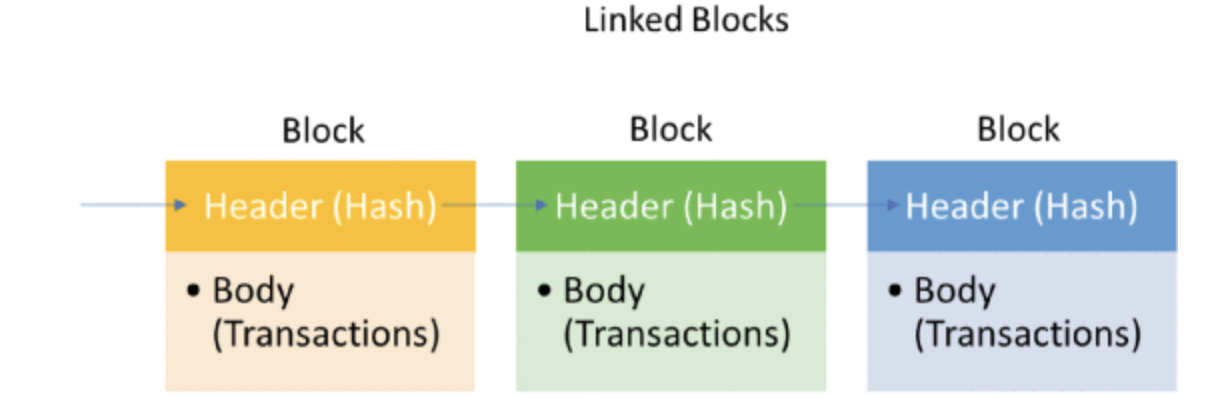
\includegraphics[width=15cm]{2-fundamentos-da-blockchain/figures/Blockchain-arch2.png}}
\caption{Blocks in the Blockchain architecture, \cite{9402747}, .}
\label{Blockchain-arquiteture}
\end{figure}

O blockchain, como mencionado anteriormente, é composto por blocos que estão interligados, permitindo o envio e recebimento de informações entre eles. Essa interconexão dos blocos forma uma rede caracterizada por nós. Existem duas categorias principais de nós: os nós completos e os nós leves. No entanto, é importante ressaltar que existem subnós que se diferenciam com base em suas funcionalidades específicas.

Os nós completos, também conhecidos como nós completos do blockchain, são responsáveis por manter uma cópia completa do registro de todas as transações ocorridas na rede blockchain. Esses nós possuem um alto nível de participação na rede e desempenham um papel crucial na validação e consenso das transações. Eles têm a capacidade de verificar todas as transações e armazenar uma cópia completa do blockchain, o que requer um grande poder de processamento e espaço de armazenamento.\cite{9402747}

Por outro lado, os nós leves, também chamados de nós-cliente, têm uma funcionalidade mais limitada em comparação aos nós completos. Esses nós não armazenam uma cópia completa do blockchain, mas apenas informações relevantes para suas operações específicas. Eles dependem dos nós completos para acessar o blockchain e verificar as transações. Os nós leves são mais leves em termos de requisitos de recursos, tornando-os adequados para dispositivos com capacidade de processamento e armazenamento limitados, como smartphones e dispositivos de IoT (Internet das Coisas).

Dentro dessas categorias, existem subnós com funcionalidades especializadas, como os nós mineradores. Os nós mineradores são responsáveis por adicionar novos blocos à cadeia, utilizando poder computacional para resolver problemas matemáticos complexos, conhecidos como prova de trabalho (proof-of-work). Eles desempenham um papel crucial na manutenção da segurança e integridade do blockchain, garantindo que apenas transações válidas sejam adicionadas aos blocos.

Essa estrutura de nós no blockchain permite a descentralização e a distribuição das informações, aumentando a segurança e a transparência do sistema. Cada nó na rede possui uma cópia do blockchain e participa da validação e consenso das transações.(Figure \ref{Blockchain-Nodes}).


\begin{figure}[!htb]
\centering
\frame{\includegraphics[width=15cm]{2-fundamentos-da-blockchain/figures/Capture d’écran 2023-12-03 à 23.07.25.png}}
\caption{Estrutua do Blockchain.}
\label{Blockchain-Nodes}
\end{figure}

			% introdução

\chapter{Fundamentos da blockchain}
\label{chapter_fondamentos}


    O Blockchain é uma tecnologia nascente de 2009, usado por Nakamoto Satoshi \cite{Blockchain-Satochi},que está transformando o mundo da tecnologia e dos negócios por sua transparência, descentralização e propriedades de segurança. Desde então, ganhou muita atenção com a sua primeira aplicação de criptomoedas, como o Bitcoin.
    
    O conceito do blockchain, que é uma palavra em inglês e significa uma cadeia de blocos, foi apresentado por STUART HABER e AL em 1991 como um meio de marcar digitalmente documentos eletrônicos com data e horas para protegê-los contra adulteração \cite{anderson2020security}. A proposta inicial do Blockchain era resolver o problema da centralização, em que se precisava de terceiros confiáveis para processar uma transação digital \cite{9402747}.

    Assim que entra em ação a função do blockchain, que é definida nesse caso como uma cadeia de blocos digitais conectados e associados uns aos outros como um livro razão distribuído aberto que armazena informações sobre as operações que estão sendo feitas dentro dos blocos. A tecnologia Blockchain é aplicada em diferentes áreas e é diversificada em vários tipos, tais como:

        - Blockchains públicos: são aqueles que estão descentralizados e permitem a integração de qualquer pessoa à rede, assim conseguindo gerenciá-los.

        - Blockchains privados: são aqueles que só aceitam a integração de pessoas de uma única rede e gerenciá-las.

        - Blockchain de consórcio: são aqueles que estão entre os blockchains públicos e privados, em termos de permissões e gerenciamento. Eles permitem a integração de pessoas de várias organizações.

    O blockchain, como o próprio nome sugere, possui uma arquitetura especial que lhe confere as características mencionadas anteriormente. Ele é projetado para armazenar informações de forma eficiente e segura entre duas partes. No blockchain, as informações são organizadas em uma lista crescente, onde cada elemento dessa lista é chamado de bloco. É essa estrutura de blocos conectados que dá ao blockchain seu nome, "cadeia de blocos".\cite{9402747}

Além disso, é importante destacar que o blockchain é descentralizado, o que significa que não é controlado por uma única entidade ou autoridade central. Em vez disso, ele é mantido e verificado por uma rede de computadores distribuídos, chamados de nós, que trabalham em conjunto para validar e registrar as transações.\cite{tapscott2016technology}

Cada bloco do blockchain contém um conjunto de transações, que podem incluir informações como data, hora, valor e identificadores das partes envolvidas. Essas transações são verificadas e validadas pelos nós da rede, garantindo a integridade e a segurança do sistema.\cite{Blockchain-Satochi}

Além disso, o blockchain utiliza técnicas criptográficas avançadas para proteger as informações armazenadas. Cada bloco possui um código único, chamado de hash, que é gerado a partir dos dados do bloco e de seu bloco anterior(Figure \ref{Blockchain-arquiteture}). Isso cria uma ligação criptográfica entre os blocos, garantindo que qualquer alteração em um bloco anterior afetaria todos os blocos subsequentes, tornando a manipulação dos dados praticamente impossível.\cite{swan2015blockchain}

\begin{figure}[!htb]
\centering
\frame{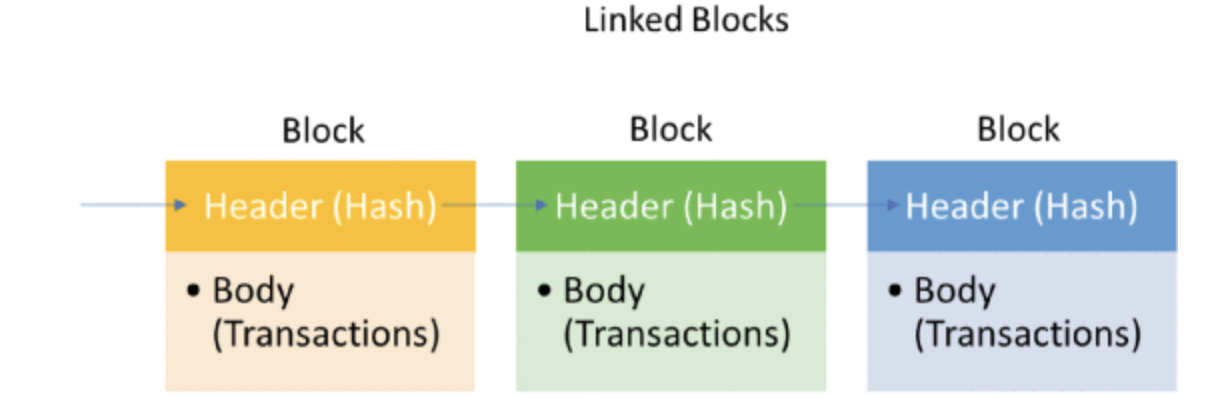
\includegraphics[width=15cm]{2-fundamentos-da-blockchain/figures/Blockchain-arch2.png}}
\caption{Blocks in the Blockchain architecture, \cite{9402747}, .}
\label{Blockchain-arquiteture}
\end{figure}

O blockchain, como mencionado anteriormente, é composto por blocos que estão interligados, permitindo o envio e recebimento de informações entre eles. Essa interconexão dos blocos forma uma rede caracterizada por nós. Existem duas categorias principais de nós: os nós completos e os nós leves. No entanto, é importante ressaltar que existem subnós que se diferenciam com base em suas funcionalidades específicas.

Os nós completos, também conhecidos como nós completos do blockchain, são responsáveis por manter uma cópia completa do registro de todas as transações ocorridas na rede blockchain. Esses nós possuem um alto nível de participação na rede e desempenham um papel crucial na validação e consenso das transações. Eles têm a capacidade de verificar todas as transações e armazenar uma cópia completa do blockchain, o que requer um grande poder de processamento e espaço de armazenamento.\cite{9402747}

Por outro lado, os nós leves, também chamados de nós-cliente, têm uma funcionalidade mais limitada em comparação aos nós completos. Esses nós não armazenam uma cópia completa do blockchain, mas apenas informações relevantes para suas operações específicas. Eles dependem dos nós completos para acessar o blockchain e verificar as transações. Os nós leves são mais leves em termos de requisitos de recursos, tornando-os adequados para dispositivos com capacidade de processamento e armazenamento limitados, como smartphones e dispositivos de IoT (Internet das Coisas).

Dentro dessas categorias, existem subnós com funcionalidades especializadas, como os nós mineradores. Os nós mineradores são responsáveis por adicionar novos blocos à cadeia, utilizando poder computacional para resolver problemas matemáticos complexos, conhecidos como prova de trabalho (proof-of-work). Eles desempenham um papel crucial na manutenção da segurança e integridade do blockchain, garantindo que apenas transações válidas sejam adicionadas aos blocos.

Essa estrutura de nós no blockchain permite a descentralização e a distribuição das informações, aumentando a segurança e a transparência do sistema. Cada nó na rede possui uma cópia do blockchain e participa da validação e consenso das transações.(Figure \ref{Blockchain-Nodes}).


\begin{figure}[!htb]
\centering
\frame{\includegraphics[width=15cm]{2-fundamentos-da-blockchain/figures/Capture d’écran 2023-12-03 à 23.07.25.png}}
\caption{Estrutua do Blockchain.}
\label{Blockchain-Nodes}
\end{figure}

   % fondamentos 

\chapter{Fundamentos da blockchain}
\label{chapter_fondamentos}


    O Blockchain é uma tecnologia nascente de 2009, usado por Nakamoto Satoshi \cite{Blockchain-Satochi},que está transformando o mundo da tecnologia e dos negócios por sua transparência, descentralização e propriedades de segurança. Desde então, ganhou muita atenção com a sua primeira aplicação de criptomoedas, como o Bitcoin.
    
    O conceito do blockchain, que é uma palavra em inglês e significa uma cadeia de blocos, foi apresentado por STUART HABER e AL em 1991 como um meio de marcar digitalmente documentos eletrônicos com data e horas para protegê-los contra adulteração \cite{anderson2020security}. A proposta inicial do Blockchain era resolver o problema da centralização, em que se precisava de terceiros confiáveis para processar uma transação digital \cite{9402747}.

    Assim que entra em ação a função do blockchain, que é definida nesse caso como uma cadeia de blocos digitais conectados e associados uns aos outros como um livro razão distribuído aberto que armazena informações sobre as operações que estão sendo feitas dentro dos blocos. A tecnologia Blockchain é aplicada em diferentes áreas e é diversificada em vários tipos, tais como:

        - Blockchains públicos: são aqueles que estão descentralizados e permitem a integração de qualquer pessoa à rede, assim conseguindo gerenciá-los.

        - Blockchains privados: são aqueles que só aceitam a integração de pessoas de uma única rede e gerenciá-las.

        - Blockchain de consórcio: são aqueles que estão entre os blockchains públicos e privados, em termos de permissões e gerenciamento. Eles permitem a integração de pessoas de várias organizações.

    O blockchain, como o próprio nome sugere, possui uma arquitetura especial que lhe confere as características mencionadas anteriormente. Ele é projetado para armazenar informações de forma eficiente e segura entre duas partes. No blockchain, as informações são organizadas em uma lista crescente, onde cada elemento dessa lista é chamado de bloco. É essa estrutura de blocos conectados que dá ao blockchain seu nome, "cadeia de blocos".\cite{9402747}

Além disso, é importante destacar que o blockchain é descentralizado, o que significa que não é controlado por uma única entidade ou autoridade central. Em vez disso, ele é mantido e verificado por uma rede de computadores distribuídos, chamados de nós, que trabalham em conjunto para validar e registrar as transações.\cite{tapscott2016technology}

Cada bloco do blockchain contém um conjunto de transações, que podem incluir informações como data, hora, valor e identificadores das partes envolvidas. Essas transações são verificadas e validadas pelos nós da rede, garantindo a integridade e a segurança do sistema.\cite{Blockchain-Satochi}

Além disso, o blockchain utiliza técnicas criptográficas avançadas para proteger as informações armazenadas. Cada bloco possui um código único, chamado de hash, que é gerado a partir dos dados do bloco e de seu bloco anterior(Figure \ref{Blockchain-arquiteture}). Isso cria uma ligação criptográfica entre os blocos, garantindo que qualquer alteração em um bloco anterior afetaria todos os blocos subsequentes, tornando a manipulação dos dados praticamente impossível.\cite{swan2015blockchain}

\begin{figure}[!htb]
\centering
\frame{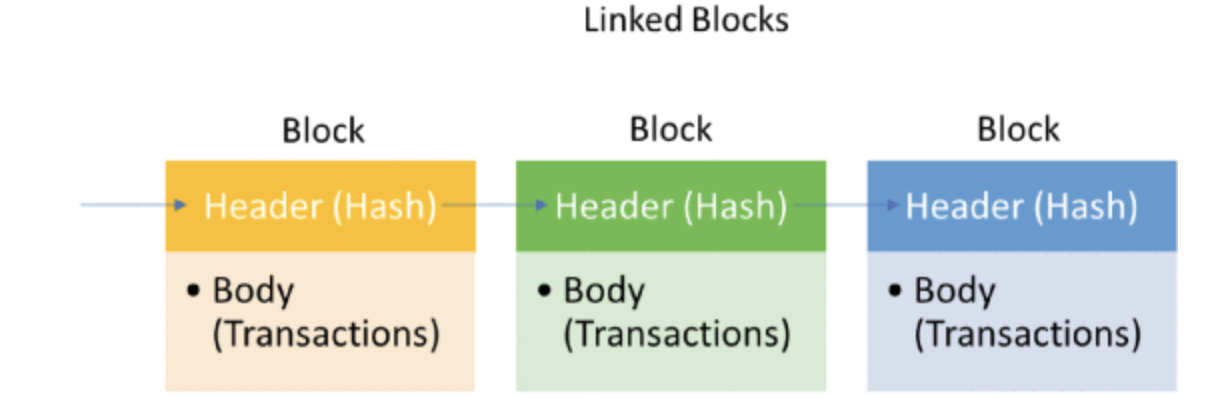
\includegraphics[width=15cm]{2-fundamentos-da-blockchain/figures/Blockchain-arch2.png}}
\caption{Blocks in the Blockchain architecture, \cite{9402747}, .}
\label{Blockchain-arquiteture}
\end{figure}

O blockchain, como mencionado anteriormente, é composto por blocos que estão interligados, permitindo o envio e recebimento de informações entre eles. Essa interconexão dos blocos forma uma rede caracterizada por nós. Existem duas categorias principais de nós: os nós completos e os nós leves. No entanto, é importante ressaltar que existem subnós que se diferenciam com base em suas funcionalidades específicas.

Os nós completos, também conhecidos como nós completos do blockchain, são responsáveis por manter uma cópia completa do registro de todas as transações ocorridas na rede blockchain. Esses nós possuem um alto nível de participação na rede e desempenham um papel crucial na validação e consenso das transações. Eles têm a capacidade de verificar todas as transações e armazenar uma cópia completa do blockchain, o que requer um grande poder de processamento e espaço de armazenamento.\cite{9402747}

Por outro lado, os nós leves, também chamados de nós-cliente, têm uma funcionalidade mais limitada em comparação aos nós completos. Esses nós não armazenam uma cópia completa do blockchain, mas apenas informações relevantes para suas operações específicas. Eles dependem dos nós completos para acessar o blockchain e verificar as transações. Os nós leves são mais leves em termos de requisitos de recursos, tornando-os adequados para dispositivos com capacidade de processamento e armazenamento limitados, como smartphones e dispositivos de IoT (Internet das Coisas).

Dentro dessas categorias, existem subnós com funcionalidades especializadas, como os nós mineradores. Os nós mineradores são responsáveis por adicionar novos blocos à cadeia, utilizando poder computacional para resolver problemas matemáticos complexos, conhecidos como prova de trabalho (proof-of-work). Eles desempenham um papel crucial na manutenção da segurança e integridade do blockchain, garantindo que apenas transações válidas sejam adicionadas aos blocos.

Essa estrutura de nós no blockchain permite a descentralização e a distribuição das informações, aumentando a segurança e a transparência do sistema. Cada nó na rede possui uma cópia do blockchain e participa da validação e consenso das transações.(Figure \ref{Blockchain-Nodes}).


\begin{figure}[!htb]
\centering
\frame{\includegraphics[width=15cm]{2-fundamentos-da-blockchain/figures/Capture d’écran 2023-12-03 à 23.07.25.png}}
\caption{Estrutua do Blockchain.}
\label{Blockchain-Nodes}
\end{figure}

 % objetivo

\chapter{Fundamentos da blockchain}
\label{chapter_fondamentos}


    O Blockchain é uma tecnologia nascente de 2009, usado por Nakamoto Satoshi \cite{Blockchain-Satochi},que está transformando o mundo da tecnologia e dos negócios por sua transparência, descentralização e propriedades de segurança. Desde então, ganhou muita atenção com a sua primeira aplicação de criptomoedas, como o Bitcoin.
    
    O conceito do blockchain, que é uma palavra em inglês e significa uma cadeia de blocos, foi apresentado por STUART HABER e AL em 1991 como um meio de marcar digitalmente documentos eletrônicos com data e horas para protegê-los contra adulteração \cite{anderson2020security}. A proposta inicial do Blockchain era resolver o problema da centralização, em que se precisava de terceiros confiáveis para processar uma transação digital \cite{9402747}.

    Assim que entra em ação a função do blockchain, que é definida nesse caso como uma cadeia de blocos digitais conectados e associados uns aos outros como um livro razão distribuído aberto que armazena informações sobre as operações que estão sendo feitas dentro dos blocos. A tecnologia Blockchain é aplicada em diferentes áreas e é diversificada em vários tipos, tais como:

        - Blockchains públicos: são aqueles que estão descentralizados e permitem a integração de qualquer pessoa à rede, assim conseguindo gerenciá-los.

        - Blockchains privados: são aqueles que só aceitam a integração de pessoas de uma única rede e gerenciá-las.

        - Blockchain de consórcio: são aqueles que estão entre os blockchains públicos e privados, em termos de permissões e gerenciamento. Eles permitem a integração de pessoas de várias organizações.

    O blockchain, como o próprio nome sugere, possui uma arquitetura especial que lhe confere as características mencionadas anteriormente. Ele é projetado para armazenar informações de forma eficiente e segura entre duas partes. No blockchain, as informações são organizadas em uma lista crescente, onde cada elemento dessa lista é chamado de bloco. É essa estrutura de blocos conectados que dá ao blockchain seu nome, "cadeia de blocos".\cite{9402747}

Além disso, é importante destacar que o blockchain é descentralizado, o que significa que não é controlado por uma única entidade ou autoridade central. Em vez disso, ele é mantido e verificado por uma rede de computadores distribuídos, chamados de nós, que trabalham em conjunto para validar e registrar as transações.\cite{tapscott2016technology}

Cada bloco do blockchain contém um conjunto de transações, que podem incluir informações como data, hora, valor e identificadores das partes envolvidas. Essas transações são verificadas e validadas pelos nós da rede, garantindo a integridade e a segurança do sistema.\cite{Blockchain-Satochi}

Além disso, o blockchain utiliza técnicas criptográficas avançadas para proteger as informações armazenadas. Cada bloco possui um código único, chamado de hash, que é gerado a partir dos dados do bloco e de seu bloco anterior(Figure \ref{Blockchain-arquiteture}). Isso cria uma ligação criptográfica entre os blocos, garantindo que qualquer alteração em um bloco anterior afetaria todos os blocos subsequentes, tornando a manipulação dos dados praticamente impossível.\cite{swan2015blockchain}

\begin{figure}[!htb]
\centering
\frame{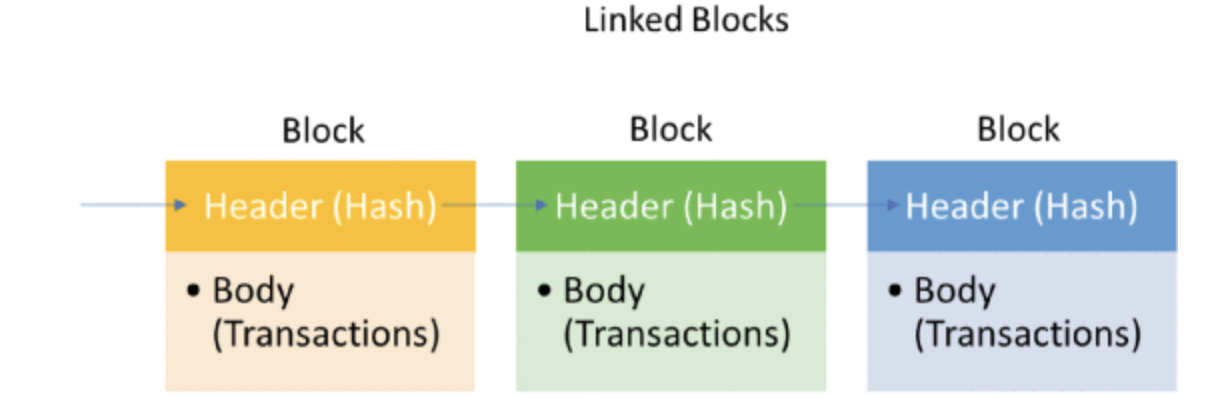
\includegraphics[width=15cm]{2-fundamentos-da-blockchain/figures/Blockchain-arch2.png}}
\caption{Blocks in the Blockchain architecture, \cite{9402747}, .}
\label{Blockchain-arquiteture}
\end{figure}

O blockchain, como mencionado anteriormente, é composto por blocos que estão interligados, permitindo o envio e recebimento de informações entre eles. Essa interconexão dos blocos forma uma rede caracterizada por nós. Existem duas categorias principais de nós: os nós completos e os nós leves. No entanto, é importante ressaltar que existem subnós que se diferenciam com base em suas funcionalidades específicas.

Os nós completos, também conhecidos como nós completos do blockchain, são responsáveis por manter uma cópia completa do registro de todas as transações ocorridas na rede blockchain. Esses nós possuem um alto nível de participação na rede e desempenham um papel crucial na validação e consenso das transações. Eles têm a capacidade de verificar todas as transações e armazenar uma cópia completa do blockchain, o que requer um grande poder de processamento e espaço de armazenamento.\cite{9402747}

Por outro lado, os nós leves, também chamados de nós-cliente, têm uma funcionalidade mais limitada em comparação aos nós completos. Esses nós não armazenam uma cópia completa do blockchain, mas apenas informações relevantes para suas operações específicas. Eles dependem dos nós completos para acessar o blockchain e verificar as transações. Os nós leves são mais leves em termos de requisitos de recursos, tornando-os adequados para dispositivos com capacidade de processamento e armazenamento limitados, como smartphones e dispositivos de IoT (Internet das Coisas).

Dentro dessas categorias, existem subnós com funcionalidades especializadas, como os nós mineradores. Os nós mineradores são responsáveis por adicionar novos blocos à cadeia, utilizando poder computacional para resolver problemas matemáticos complexos, conhecidos como prova de trabalho (proof-of-work). Eles desempenham um papel crucial na manutenção da segurança e integridade do blockchain, garantindo que apenas transações válidas sejam adicionadas aos blocos.

Essa estrutura de nós no blockchain permite a descentralização e a distribuição das informações, aumentando a segurança e a transparência do sistema. Cada nó na rede possui uma cópia do blockchain e participa da validação e consenso das transações.(Figure \ref{Blockchain-Nodes}).


\begin{figure}[!htb]
\centering
\frame{\includegraphics[width=15cm]{2-fundamentos-da-blockchain/figures/Capture d’écran 2023-12-03 à 23.07.25.png}}
\caption{Estrutua do Blockchain.}
\label{Blockchain-Nodes}
\end{figure}

 % analise de desempenho

\chapter{Fundamentos da blockchain}
\label{chapter_fondamentos}


    O Blockchain é uma tecnologia nascente de 2009, usado por Nakamoto Satoshi \cite{Blockchain-Satochi},que está transformando o mundo da tecnologia e dos negócios por sua transparência, descentralização e propriedades de segurança. Desde então, ganhou muita atenção com a sua primeira aplicação de criptomoedas, como o Bitcoin.
    
    O conceito do blockchain, que é uma palavra em inglês e significa uma cadeia de blocos, foi apresentado por STUART HABER e AL em 1991 como um meio de marcar digitalmente documentos eletrônicos com data e horas para protegê-los contra adulteração \cite{anderson2020security}. A proposta inicial do Blockchain era resolver o problema da centralização, em que se precisava de terceiros confiáveis para processar uma transação digital \cite{9402747}.

    Assim que entra em ação a função do blockchain, que é definida nesse caso como uma cadeia de blocos digitais conectados e associados uns aos outros como um livro razão distribuído aberto que armazena informações sobre as operações que estão sendo feitas dentro dos blocos. A tecnologia Blockchain é aplicada em diferentes áreas e é diversificada em vários tipos, tais como:

        - Blockchains públicos: são aqueles que estão descentralizados e permitem a integração de qualquer pessoa à rede, assim conseguindo gerenciá-los.

        - Blockchains privados: são aqueles que só aceitam a integração de pessoas de uma única rede e gerenciá-las.

        - Blockchain de consórcio: são aqueles que estão entre os blockchains públicos e privados, em termos de permissões e gerenciamento. Eles permitem a integração de pessoas de várias organizações.

    O blockchain, como o próprio nome sugere, possui uma arquitetura especial que lhe confere as características mencionadas anteriormente. Ele é projetado para armazenar informações de forma eficiente e segura entre duas partes. No blockchain, as informações são organizadas em uma lista crescente, onde cada elemento dessa lista é chamado de bloco. É essa estrutura de blocos conectados que dá ao blockchain seu nome, "cadeia de blocos".\cite{9402747}

Além disso, é importante destacar que o blockchain é descentralizado, o que significa que não é controlado por uma única entidade ou autoridade central. Em vez disso, ele é mantido e verificado por uma rede de computadores distribuídos, chamados de nós, que trabalham em conjunto para validar e registrar as transações.\cite{tapscott2016technology}

Cada bloco do blockchain contém um conjunto de transações, que podem incluir informações como data, hora, valor e identificadores das partes envolvidas. Essas transações são verificadas e validadas pelos nós da rede, garantindo a integridade e a segurança do sistema.\cite{Blockchain-Satochi}

Além disso, o blockchain utiliza técnicas criptográficas avançadas para proteger as informações armazenadas. Cada bloco possui um código único, chamado de hash, que é gerado a partir dos dados do bloco e de seu bloco anterior(Figure \ref{Blockchain-arquiteture}). Isso cria uma ligação criptográfica entre os blocos, garantindo que qualquer alteração em um bloco anterior afetaria todos os blocos subsequentes, tornando a manipulação dos dados praticamente impossível.\cite{swan2015blockchain}

\begin{figure}[!htb]
\centering
\frame{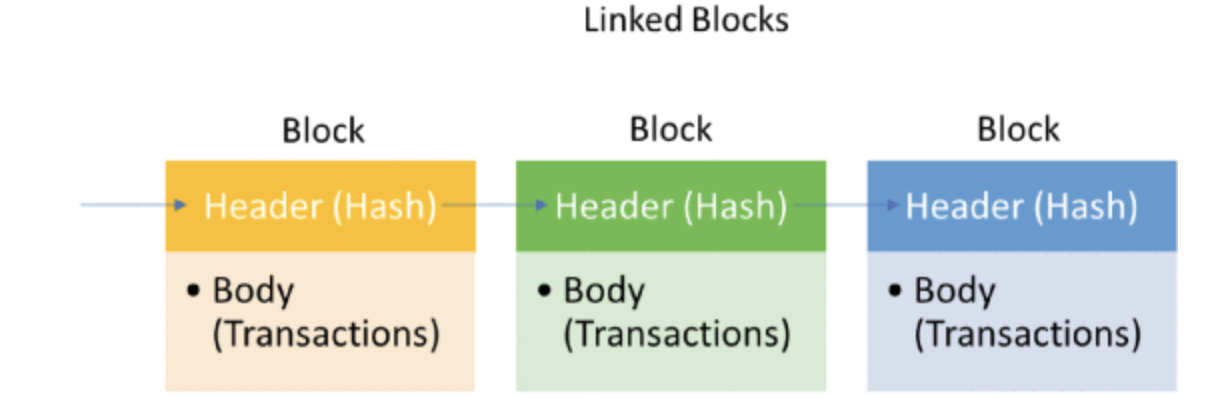
\includegraphics[width=15cm]{2-fundamentos-da-blockchain/figures/Blockchain-arch2.png}}
\caption{Blocks in the Blockchain architecture, \cite{9402747}, .}
\label{Blockchain-arquiteture}
\end{figure}

O blockchain, como mencionado anteriormente, é composto por blocos que estão interligados, permitindo o envio e recebimento de informações entre eles. Essa interconexão dos blocos forma uma rede caracterizada por nós. Existem duas categorias principais de nós: os nós completos e os nós leves. No entanto, é importante ressaltar que existem subnós que se diferenciam com base em suas funcionalidades específicas.

Os nós completos, também conhecidos como nós completos do blockchain, são responsáveis por manter uma cópia completa do registro de todas as transações ocorridas na rede blockchain. Esses nós possuem um alto nível de participação na rede e desempenham um papel crucial na validação e consenso das transações. Eles têm a capacidade de verificar todas as transações e armazenar uma cópia completa do blockchain, o que requer um grande poder de processamento e espaço de armazenamento.\cite{9402747}

Por outro lado, os nós leves, também chamados de nós-cliente, têm uma funcionalidade mais limitada em comparação aos nós completos. Esses nós não armazenam uma cópia completa do blockchain, mas apenas informações relevantes para suas operações específicas. Eles dependem dos nós completos para acessar o blockchain e verificar as transações. Os nós leves são mais leves em termos de requisitos de recursos, tornando-os adequados para dispositivos com capacidade de processamento e armazenamento limitados, como smartphones e dispositivos de IoT (Internet das Coisas).

Dentro dessas categorias, existem subnós com funcionalidades especializadas, como os nós mineradores. Os nós mineradores são responsáveis por adicionar novos blocos à cadeia, utilizando poder computacional para resolver problemas matemáticos complexos, conhecidos como prova de trabalho (proof-of-work). Eles desempenham um papel crucial na manutenção da segurança e integridade do blockchain, garantindo que apenas transações válidas sejam adicionadas aos blocos.

Essa estrutura de nós no blockchain permite a descentralização e a distribuição das informações, aumentando a segurança e a transparência do sistema. Cada nó na rede possui uma cópia do blockchain e participa da validação e consenso das transações.(Figure \ref{Blockchain-Nodes}).


\begin{figure}[!htb]
\centering
\frame{\includegraphics[width=15cm]{2-fundamentos-da-blockchain/figures/Capture d’écran 2023-12-03 à 23.07.25.png}}
\caption{Estrutua do Blockchain.}
\label{Blockchain-Nodes}
\end{figure}

   % experimentos

\chapter{Fundamentos da blockchain}
\label{chapter_fondamentos}


    O Blockchain é uma tecnologia nascente de 2009, usado por Nakamoto Satoshi \cite{Blockchain-Satochi},que está transformando o mundo da tecnologia e dos negócios por sua transparência, descentralização e propriedades de segurança. Desde então, ganhou muita atenção com a sua primeira aplicação de criptomoedas, como o Bitcoin.
    
    O conceito do blockchain, que é uma palavra em inglês e significa uma cadeia de blocos, foi apresentado por STUART HABER e AL em 1991 como um meio de marcar digitalmente documentos eletrônicos com data e horas para protegê-los contra adulteração \cite{anderson2020security}. A proposta inicial do Blockchain era resolver o problema da centralização, em que se precisava de terceiros confiáveis para processar uma transação digital \cite{9402747}.

    Assim que entra em ação a função do blockchain, que é definida nesse caso como uma cadeia de blocos digitais conectados e associados uns aos outros como um livro razão distribuído aberto que armazena informações sobre as operações que estão sendo feitas dentro dos blocos. A tecnologia Blockchain é aplicada em diferentes áreas e é diversificada em vários tipos, tais como:

        - Blockchains públicos: são aqueles que estão descentralizados e permitem a integração de qualquer pessoa à rede, assim conseguindo gerenciá-los.

        - Blockchains privados: são aqueles que só aceitam a integração de pessoas de uma única rede e gerenciá-las.

        - Blockchain de consórcio: são aqueles que estão entre os blockchains públicos e privados, em termos de permissões e gerenciamento. Eles permitem a integração de pessoas de várias organizações.

    O blockchain, como o próprio nome sugere, possui uma arquitetura especial que lhe confere as características mencionadas anteriormente. Ele é projetado para armazenar informações de forma eficiente e segura entre duas partes. No blockchain, as informações são organizadas em uma lista crescente, onde cada elemento dessa lista é chamado de bloco. É essa estrutura de blocos conectados que dá ao blockchain seu nome, "cadeia de blocos".\cite{9402747}

Além disso, é importante destacar que o blockchain é descentralizado, o que significa que não é controlado por uma única entidade ou autoridade central. Em vez disso, ele é mantido e verificado por uma rede de computadores distribuídos, chamados de nós, que trabalham em conjunto para validar e registrar as transações.\cite{tapscott2016technology}

Cada bloco do blockchain contém um conjunto de transações, que podem incluir informações como data, hora, valor e identificadores das partes envolvidas. Essas transações são verificadas e validadas pelos nós da rede, garantindo a integridade e a segurança do sistema.\cite{Blockchain-Satochi}

Além disso, o blockchain utiliza técnicas criptográficas avançadas para proteger as informações armazenadas. Cada bloco possui um código único, chamado de hash, que é gerado a partir dos dados do bloco e de seu bloco anterior(Figure \ref{Blockchain-arquiteture}). Isso cria uma ligação criptográfica entre os blocos, garantindo que qualquer alteração em um bloco anterior afetaria todos os blocos subsequentes, tornando a manipulação dos dados praticamente impossível.\cite{swan2015blockchain}

\begin{figure}[!htb]
\centering
\frame{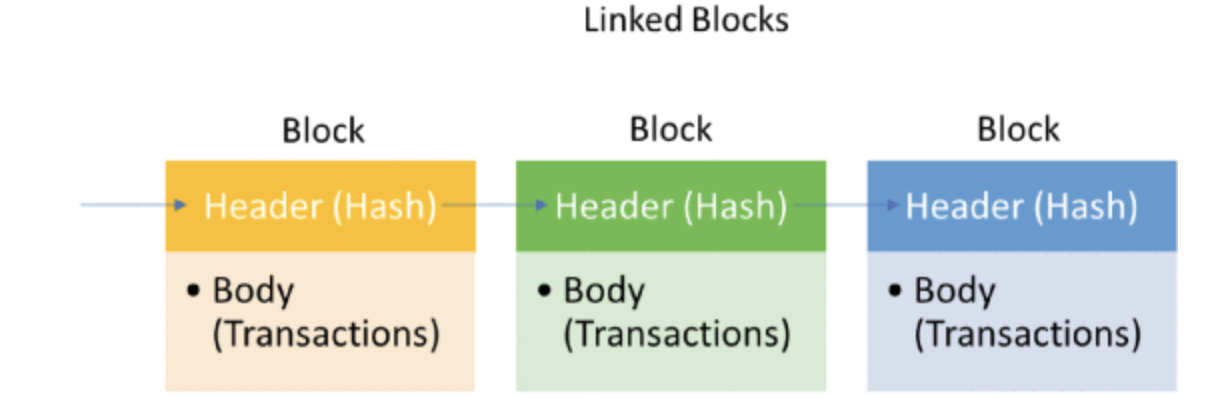
\includegraphics[width=15cm]{2-fundamentos-da-blockchain/figures/Blockchain-arch2.png}}
\caption{Blocks in the Blockchain architecture, \cite{9402747}, .}
\label{Blockchain-arquiteture}
\end{figure}

O blockchain, como mencionado anteriormente, é composto por blocos que estão interligados, permitindo o envio e recebimento de informações entre eles. Essa interconexão dos blocos forma uma rede caracterizada por nós. Existem duas categorias principais de nós: os nós completos e os nós leves. No entanto, é importante ressaltar que existem subnós que se diferenciam com base em suas funcionalidades específicas.

Os nós completos, também conhecidos como nós completos do blockchain, são responsáveis por manter uma cópia completa do registro de todas as transações ocorridas na rede blockchain. Esses nós possuem um alto nível de participação na rede e desempenham um papel crucial na validação e consenso das transações. Eles têm a capacidade de verificar todas as transações e armazenar uma cópia completa do blockchain, o que requer um grande poder de processamento e espaço de armazenamento.\cite{9402747}

Por outro lado, os nós leves, também chamados de nós-cliente, têm uma funcionalidade mais limitada em comparação aos nós completos. Esses nós não armazenam uma cópia completa do blockchain, mas apenas informações relevantes para suas operações específicas. Eles dependem dos nós completos para acessar o blockchain e verificar as transações. Os nós leves são mais leves em termos de requisitos de recursos, tornando-os adequados para dispositivos com capacidade de processamento e armazenamento limitados, como smartphones e dispositivos de IoT (Internet das Coisas).

Dentro dessas categorias, existem subnós com funcionalidades especializadas, como os nós mineradores. Os nós mineradores são responsáveis por adicionar novos blocos à cadeia, utilizando poder computacional para resolver problemas matemáticos complexos, conhecidos como prova de trabalho (proof-of-work). Eles desempenham um papel crucial na manutenção da segurança e integridade do blockchain, garantindo que apenas transações válidas sejam adicionadas aos blocos.

Essa estrutura de nós no blockchain permite a descentralização e a distribuição das informações, aumentando a segurança e a transparência do sistema. Cada nó na rede possui uma cópia do blockchain e participa da validação e consenso das transações.(Figure \ref{Blockchain-Nodes}).


\begin{figure}[!htb]
\centering
\frame{\includegraphics[width=15cm]{2-fundamentos-da-blockchain/figures/Capture d’écran 2023-12-03 à 23.07.25.png}}
\caption{Estrutua do Blockchain.}
\label{Blockchain-Nodes}
\end{figure}



\chapter{Fundamentos da blockchain}
\label{chapter_fondamentos}


    O Blockchain é uma tecnologia nascente de 2009, usado por Nakamoto Satoshi \cite{Blockchain-Satochi},que está transformando o mundo da tecnologia e dos negócios por sua transparência, descentralização e propriedades de segurança. Desde então, ganhou muita atenção com a sua primeira aplicação de criptomoedas, como o Bitcoin.
    
    O conceito do blockchain, que é uma palavra em inglês e significa uma cadeia de blocos, foi apresentado por STUART HABER e AL em 1991 como um meio de marcar digitalmente documentos eletrônicos com data e horas para protegê-los contra adulteração \cite{anderson2020security}. A proposta inicial do Blockchain era resolver o problema da centralização, em que se precisava de terceiros confiáveis para processar uma transação digital \cite{9402747}.

    Assim que entra em ação a função do blockchain, que é definida nesse caso como uma cadeia de blocos digitais conectados e associados uns aos outros como um livro razão distribuído aberto que armazena informações sobre as operações que estão sendo feitas dentro dos blocos. A tecnologia Blockchain é aplicada em diferentes áreas e é diversificada em vários tipos, tais como:

        - Blockchains públicos: são aqueles que estão descentralizados e permitem a integração de qualquer pessoa à rede, assim conseguindo gerenciá-los.

        - Blockchains privados: são aqueles que só aceitam a integração de pessoas de uma única rede e gerenciá-las.

        - Blockchain de consórcio: são aqueles que estão entre os blockchains públicos e privados, em termos de permissões e gerenciamento. Eles permitem a integração de pessoas de várias organizações.

    O blockchain, como o próprio nome sugere, possui uma arquitetura especial que lhe confere as características mencionadas anteriormente. Ele é projetado para armazenar informações de forma eficiente e segura entre duas partes. No blockchain, as informações são organizadas em uma lista crescente, onde cada elemento dessa lista é chamado de bloco. É essa estrutura de blocos conectados que dá ao blockchain seu nome, "cadeia de blocos".\cite{9402747}

Além disso, é importante destacar que o blockchain é descentralizado, o que significa que não é controlado por uma única entidade ou autoridade central. Em vez disso, ele é mantido e verificado por uma rede de computadores distribuídos, chamados de nós, que trabalham em conjunto para validar e registrar as transações.\cite{tapscott2016technology}

Cada bloco do blockchain contém um conjunto de transações, que podem incluir informações como data, hora, valor e identificadores das partes envolvidas. Essas transações são verificadas e validadas pelos nós da rede, garantindo a integridade e a segurança do sistema.\cite{Blockchain-Satochi}

Além disso, o blockchain utiliza técnicas criptográficas avançadas para proteger as informações armazenadas. Cada bloco possui um código único, chamado de hash, que é gerado a partir dos dados do bloco e de seu bloco anterior(Figure \ref{Blockchain-arquiteture}). Isso cria uma ligação criptográfica entre os blocos, garantindo que qualquer alteração em um bloco anterior afetaria todos os blocos subsequentes, tornando a manipulação dos dados praticamente impossível.\cite{swan2015blockchain}

\begin{figure}[!htb]
\centering
\frame{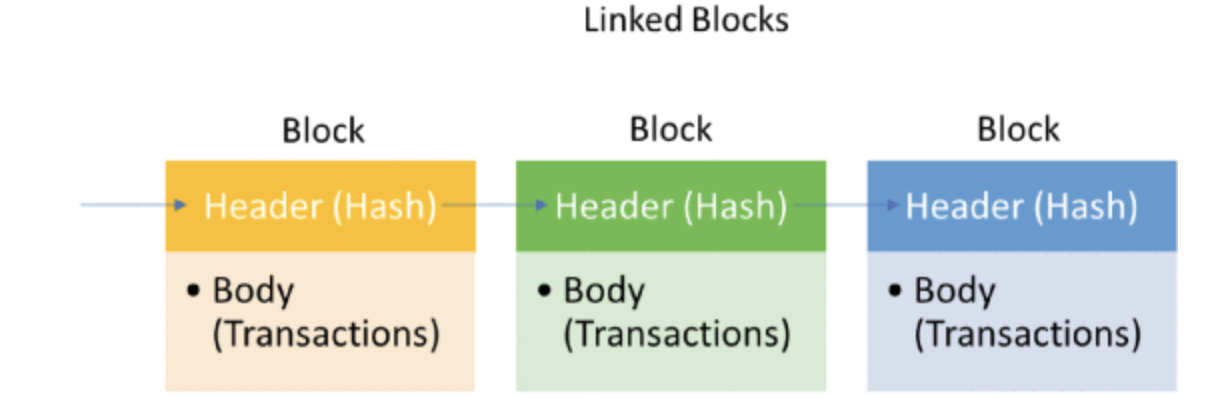
\includegraphics[width=15cm]{2-fundamentos-da-blockchain/figures/Blockchain-arch2.png}}
\caption{Blocks in the Blockchain architecture, \cite{9402747}, .}
\label{Blockchain-arquiteture}
\end{figure}

O blockchain, como mencionado anteriormente, é composto por blocos que estão interligados, permitindo o envio e recebimento de informações entre eles. Essa interconexão dos blocos forma uma rede caracterizada por nós. Existem duas categorias principais de nós: os nós completos e os nós leves. No entanto, é importante ressaltar que existem subnós que se diferenciam com base em suas funcionalidades específicas.

Os nós completos, também conhecidos como nós completos do blockchain, são responsáveis por manter uma cópia completa do registro de todas as transações ocorridas na rede blockchain. Esses nós possuem um alto nível de participação na rede e desempenham um papel crucial na validação e consenso das transações. Eles têm a capacidade de verificar todas as transações e armazenar uma cópia completa do blockchain, o que requer um grande poder de processamento e espaço de armazenamento.\cite{9402747}

Por outro lado, os nós leves, também chamados de nós-cliente, têm uma funcionalidade mais limitada em comparação aos nós completos. Esses nós não armazenam uma cópia completa do blockchain, mas apenas informações relevantes para suas operações específicas. Eles dependem dos nós completos para acessar o blockchain e verificar as transações. Os nós leves são mais leves em termos de requisitos de recursos, tornando-os adequados para dispositivos com capacidade de processamento e armazenamento limitados, como smartphones e dispositivos de IoT (Internet das Coisas).

Dentro dessas categorias, existem subnós com funcionalidades especializadas, como os nós mineradores. Os nós mineradores são responsáveis por adicionar novos blocos à cadeia, utilizando poder computacional para resolver problemas matemáticos complexos, conhecidos como prova de trabalho (proof-of-work). Eles desempenham um papel crucial na manutenção da segurança e integridade do blockchain, garantindo que apenas transações válidas sejam adicionadas aos blocos.

Essa estrutura de nós no blockchain permite a descentralização e a distribuição das informações, aumentando a segurança e a transparência do sistema. Cada nó na rede possui uma cópia do blockchain e participa da validação e consenso das transações.(Figure \ref{Blockchain-Nodes}).


\begin{figure}[!htb]
\centering
\frame{\includegraphics[width=15cm]{2-fundamentos-da-blockchain/figures/Capture d’écran 2023-12-03 à 23.07.25.png}}
\caption{Estrutua do Blockchain.}
\label{Blockchain-Nodes}
\end{figure}




%\bibliographystyle{alpha}
%\bibliography{sample}


%=====================================================

% o estilo de bibliografia é definido no arquivo packages.tex

% ATENÇÃO: evite usar \cite{}; prefira \citep{} e \citet{}

% base de bibliografia (BibTeX)

\bibliography{referencias}
\nocite{*}
%\bibliography{file1,file2,file3} % se tiver mais de um arquivo BibTeX

%=====================================================

\end{document}